
\chapter{System design}
\section{System overview} \label{sec:system}
The following system is a smart power meter with the ability to measure voltage, current and phase shift for a switchable AC line. This system operated from a \SI{240}{VAC} power source stepped down to \SI{24}{VAC}/\SI{18}{VAC} to ensure safe operation, with all of the signal measurements and trip status information and override reported to the user in the form of a GUI via an Arduino compatible microcontroller. This complex system was implemented and tested modularly to ensure successful operation of all components in the final integrated system. Figure \ref{fig:system_diagram} displays the subsystems of the final design and the interaction of these systems to meet all of the design requirements.

\subsection{Power supply}\label{subsec:power}
A power regulation system compatible with both \SI{24}{VAC}/\SI{18}{VAC} input voltages was designed as the first part of this system. The high voltage \SI{240}{VAC} input to the transformer was stepped down to \SI{24}{VAC}/\SI{18}{VAC}, with a \SI{500}{\milli A} fuse for extreme over-current protection. This output voltage was to be used to supply a load with a maximum current draw of \SI{200}{\milli A}, it was also rectified to be used by the intermediary \SI{12}{V} stage. This intermediary stage was necessary as to power the \SI{+5}{V} and \SI{-5}{V} regulators which had a relatively low maximum input voltage. These low voltage regulators were implemented using a linear regulator and a charge pump respectively, with the \SI{+5}{V} and \SI{-5}{V} supplies used to power the rail voltages of the operational amplifier and trip switch circuitry.

\subsection{Signal conditioning}\label{subsec:signal}
A signal conditioning system capable of measuring voltages and currents as well as the phase differences between these sinusoidal signals makes up the second part of this system. Load voltage levels were rectified and stepped down using a voltage divider before measurements, and the current through the load was measured by amplifying the voltage over a sense resistor in series with the load. Phase differences were measured by using the voltage and current signals in conjunction with comparators and a XOR gate to generate a PWM signal, this PWM signal was then scaled to a voltage level by using a simple low pass filter. To keep the design simplistic and the measurement circuitry reliable, only the \SI{5}{\volt} rail was used to supply the positive rail of the operational amplifiers, with these operational amplifiers all used in the single supply configuration. The signal conditioning circuitry utilized the TLC2272 rail to rail operational amplifiers as to maximise the accuracy of the reported measurements as well as to keep the total supply current draw from the \SI{5}{\volt} regulator to a minimum of \SI{22}{\milli A}.

\subsection{Over-current protection}\label{subsec:protect}
A protection system capable of controlling the \SI{24}{VAC}/\SI{18}{VAC} supply to the load and displaying critical load measurements to the user makes up the final part of this system. The purpose of this switch is to turn off the supply to the load when an over current condition is detected and to protect against overvoltage during switching. Overcurrent detection was achieved by utilising the current transducer discussed in Subsection \ref{subsec:signal} as well as a SR latch that would latch to a logical high once the overcurrent condition was triggered. This overcurrent condition would remove the voltage to the load through the use of a triac and the supply voltage could be reset via a GUI, with added switching overvoltage protection achieved by using a TVS diode.

\begin{figure}[h]
    \centering
    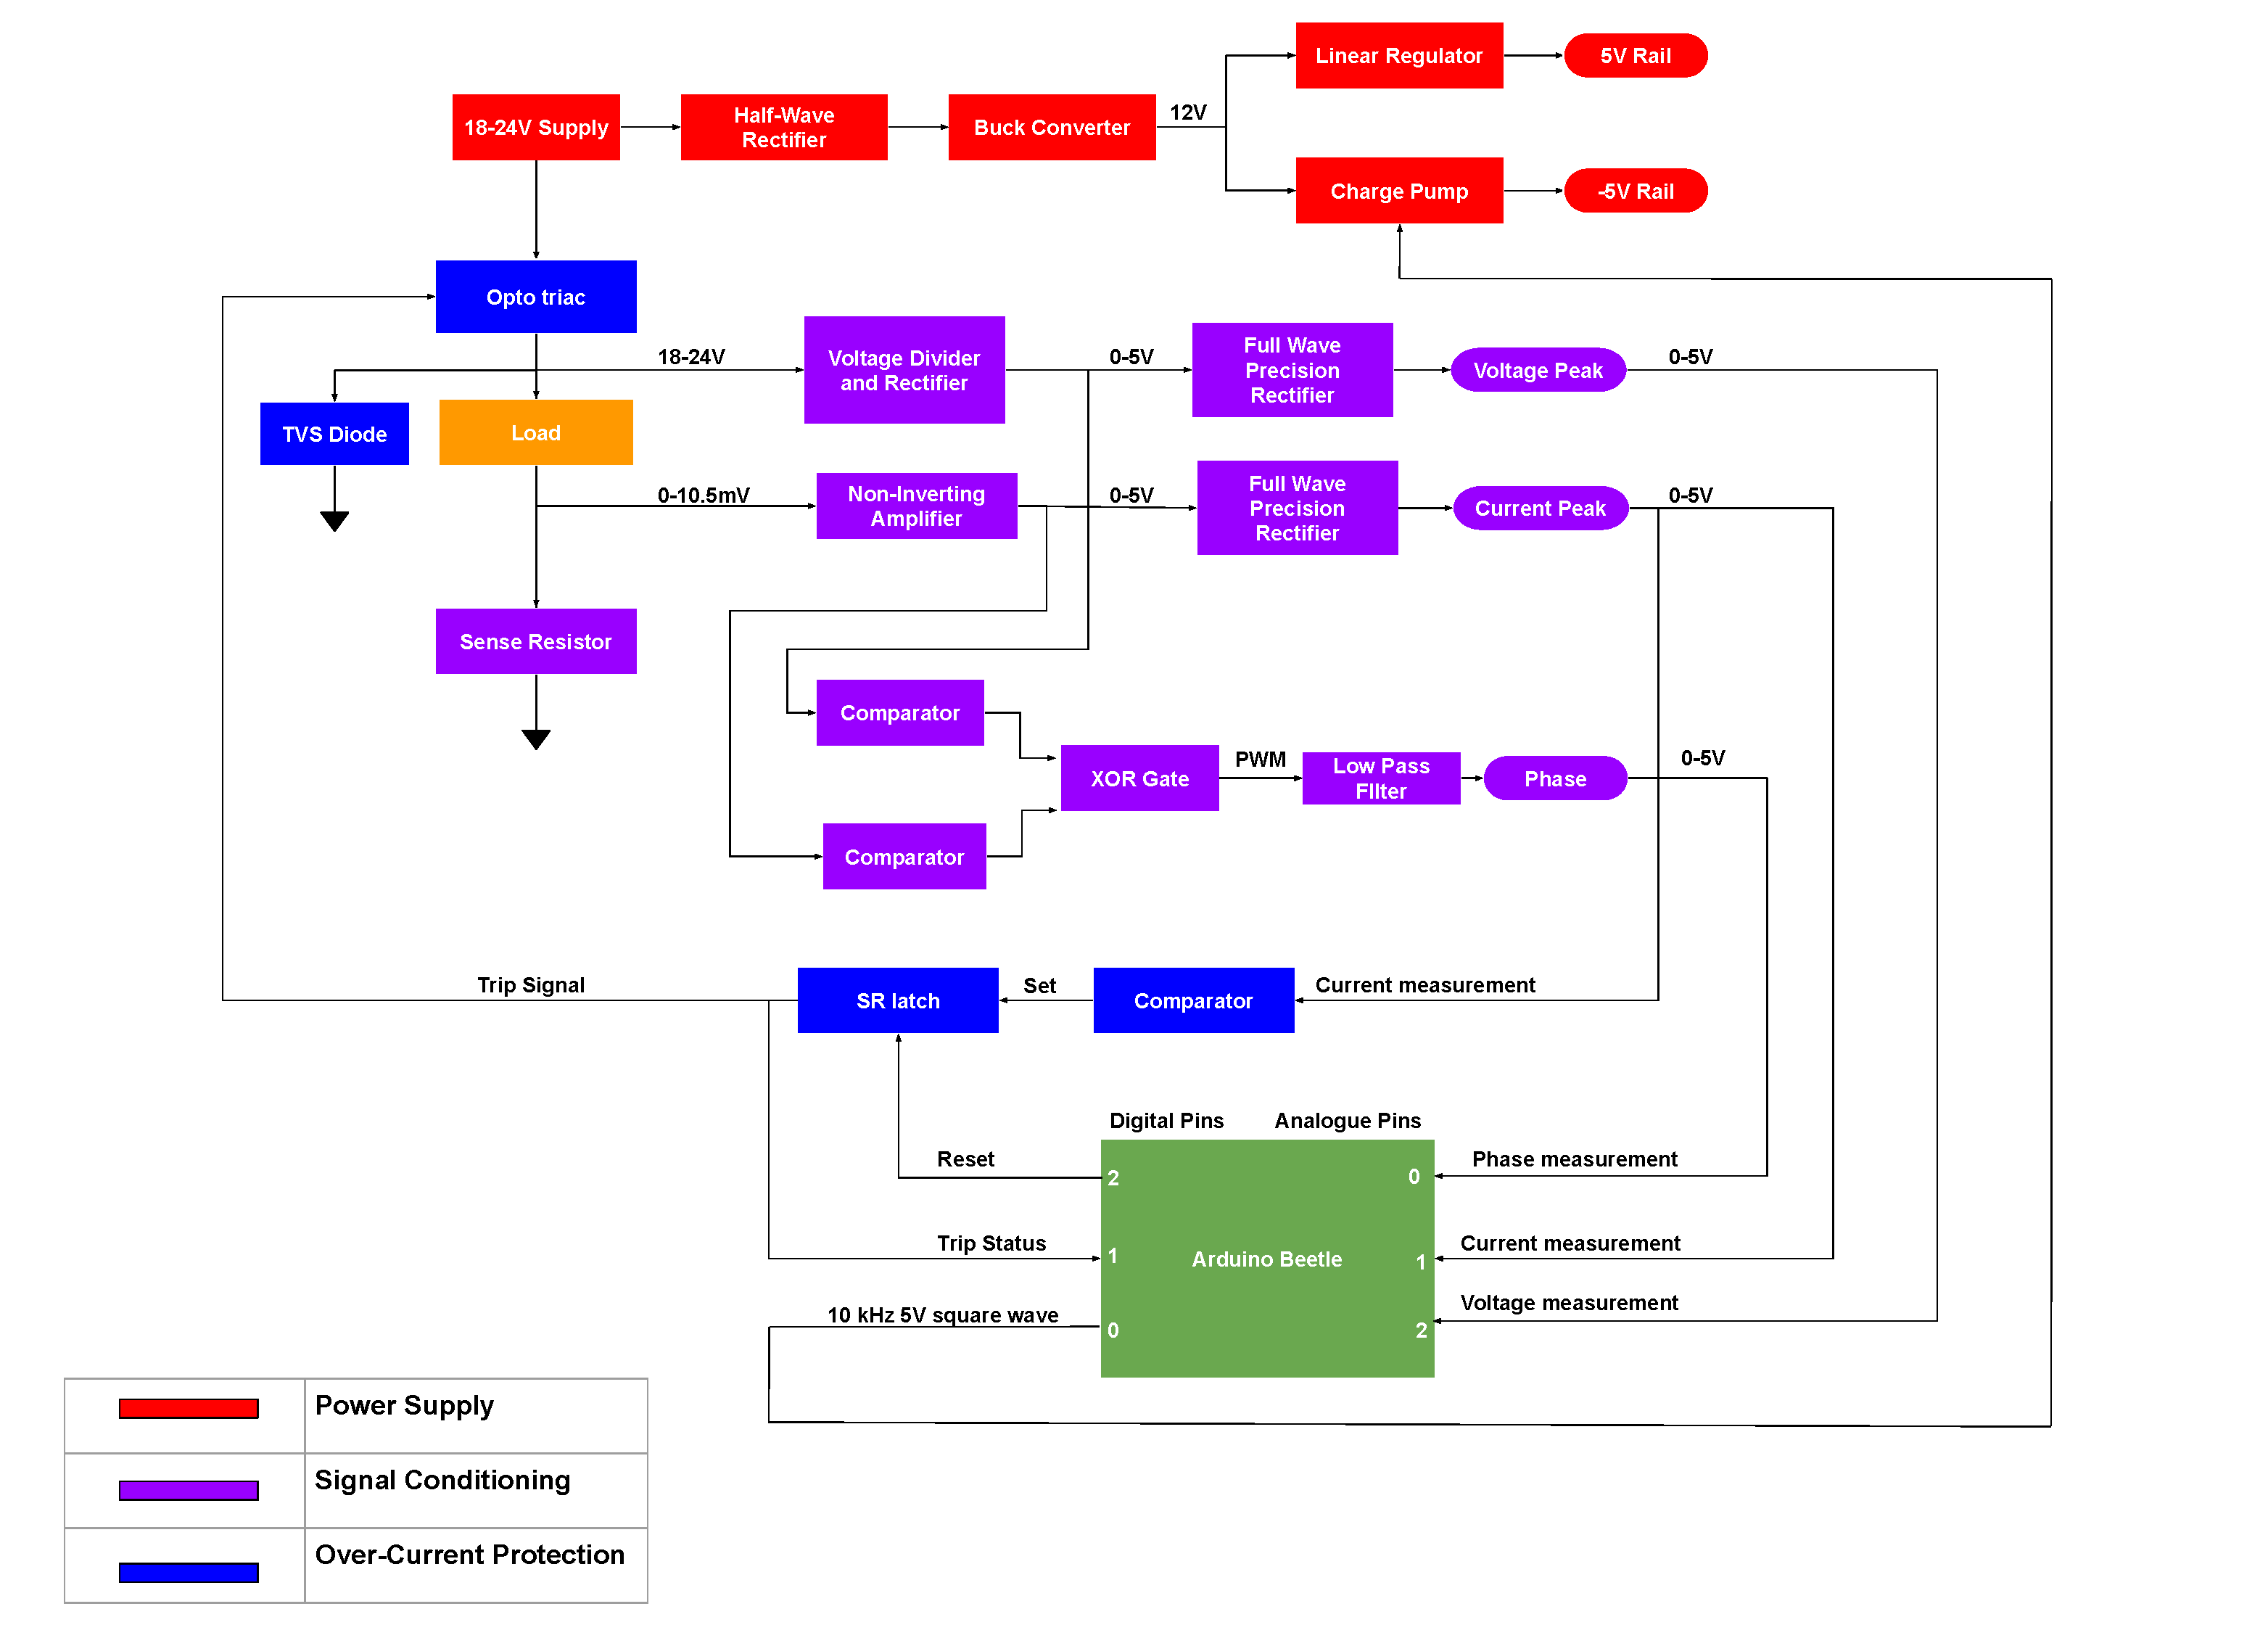
\includegraphics[width = 1\linewidth]{Figures/system_diagram.pdf}
    \caption{System diagram}
    \label{fig:system_diagram}
\end{figure}











